\documentclass[]{article}
% includes
\usepackage{amsmath}
\usepackage{amsthm}
\usepackage{amssymb}
\usepackage{authblk}
\usepackage{mathtools}
\usepackage{makecell}
\usepackage{physics}
\usepackage{hyperref}
\usepackage{bm}\newcommand{\ind}{\bm{1}}
\usepackage{multirow}
\usepackage[table]{xcolor}
\usepackage{booktabs}
\usepackage[utf8]{inputenc}
\usepackage{adjustbox}
\usepackage{caption}\captionsetup[table]{skip=1em}
\usepackage{rotating}
\usepackage{graphicx}
\graphicspath{{fig/}}
\usepackage[margin=3cm]{geometry}

% definitions
\DeclarePairedDelimiter{\floor}{\lfloor}{\rfloor}
\DeclarePairedDelimiter{\ceil}{\lceil}{\rceil}
\DeclareUnicodeCharacter{2713}{\checkmark}
\setlength{\parskip}{1em}

\makeatletter
\newcommand{\printfnsymbol}[1]{%
	\textsuperscript{\@fnsymbol{#1}}%
}
\makeatother

\makeatletter
\def\blfootnote{\gdef\@thefnmark{}\@footnotetext}
\makeatother

% Keywords command
\providecommand{\keywords}[1]
{
	\small	
	\textbf{\textit{Keywords:}} #1
}
%\DeclarePairedDelimiter{\floor}{\lfloor}{\rfloor}
\DeclarePairedDelimiter{\ceil}{\lceil}{\rceil}
\newcommand{\ind}{\mathbbm{1}}

\title{A flexible integer linear programming formulation for scheduling
	clinician on-call service in hospitals}

\author[a, b]{David Landsman}
\author[a]{Huiting Ma}
\author[a]{Jesse Knight}
\author[c]{Kevin Gough}
\author[a, c, d, e]{Sharmistha Mishra}

\renewcommand\Affilfont{\itshape\small}
\affil[a]{MAP Centre for Urban Health Solutions, Unity Health Toronto, Toronto,
	ON, Canada}
\affil[b]{Department of Computer Science, University of Toronto, Toronto, ON,
	Canada}
\affil[c]{Department of Medicine, Division of Infectious Disease, St.\ Michael's
	Hospital, University of Toronto, Toronto, ON, Canada}
\affil[d]{Institute of Health Policy, Management and Evaluation, Dalla Lana
	School of Public Health, University of Toronto, Toronto, ON, Canada}
\affil[e]{Institute of Medical Sciences, University of Toronto, Toronto, ON,
	Canada}

\begin{document}
	\maketitle
	
	\begin{abstract}
		Scheduling of personnel in a hospital environment is vital to improving the service provided to patients and balancing the workload assigned to clinicians. Many approaches have been tried and successfully applied to generate efficient schedules in such settings. However, due to the computational complexity of the scheduling problem in general, most approaches resort to heuristics to find a non-optimal solution in a reasonable amount of time. We designed an integer linear programming formulation to find an optimal schedule in a clinical division of a hospital. It mitigates computational complexity issues by maintaining a minimal set of constraints, yet still provides the flexibility necessary to adapt the formulation to a variety of clinical divisions. \\

We then conducted a case study for our approach using data from the Infectious Diseases division at St. Michael's Hospital in Toronto, Canada. We analyzed and compared the results of our approach to manually-created schedules at the hospital, and found improved adherence to departmental constraints and clinician preferences. We then used simulated data to examine the the sensitivity of the runtime of our linear program for various parameters and observed reassuring results, signifying the practicality and generazability of our approach in different real-world scenarios.
	\end{abstract}
	
	\section{Introduction}\label{sec:introduction}
	Hospital departments must allocate and use their limited resources efficiently
in order to provide a high quality of care for their patients.
In particular, on-call schedules for
a fixed number of health-care providers are central to the efficient running of
hospitals. Carefully allocated schedules should balance
sufficient staff with workload
to maximize quality of care. It is common for on-call schedules in
hospitals to be created manually. However,
manually-created schedules are subject to three problems.
First, when there are a large number of clinicians,
or the constraints that need to be satisfied
by the schedule are complex, it becomes infeasible
to find a satisfying schedule by hand. 
Second, when creating a schedule manually it is difficult to ensure
that all constraints are met while also trying to satisfy all staff
preferences.
Third, manual scheduling is often time-consuming even for relatively small 
departments, and can take up time and resources that are better used
for improving patient care.
For these reasons, it is important to develop automated methods that
can efficiently generate schedules that satisfy the given constraints.

Automated methods to generate schedules have been studied and applied in many
industries, including
transportation~\cite{aickelin_improved_2006, goel_truck_2012, gunther_combined_2010},
manufacturing~\cite{al-yakoob_mixed-integer_2007, al-yakoob_column_2008, alfares_simulation_2007},
retail~\cite{chapados_retail_2011, nissen_automatic_2010}, and
military~\cite{horn_scheduling_2007, laguna_modeling_2005}.
Of special interest to a clinician scheduling
problem are the approaches to scheduling nurses, who often work in shifts. In the
nurse scheduling problem, the goal is to find an optimal assignment of nurses to
shifts that satisfies all hard constraints (such as hospital regulations),
and as many soft constraints (such as nurse preferences) as possible.
Hard constraints must be satisfied by any candidate solution to the nurse scheduling problem,
while soft constraints can be used to rank the candidate solutions. 
For instance, a nurse scheduling problem may include a hard constraint to assign
at most a single shift for each nurse per day. It can also incorporate 
nurse preference for shift time (that is, day versus night shifts) as a soft constraint
that is meant to optimize the schedule, but is not guaranteed to be fulfilled.
A wide variety of approaches, including exact and heuristic approaches, have been
used to solve the nurse scheduling problem:
integer linear programming~\cite{azaiez_0-1_2005, trilling_nurse_2006, widyastiti_nurses_2016},
network flows~\cite{el_adoly_new_2018},
genetic algorithms~\cite{aickelin_exploiting_2000, jan_evolutionary_2000, kawanaka_genetic_2001},
simulated annealing~\cite{jaszkiewicz_metaheuristic_1997}, and
artificial intelligence~\cite{abdennadher_nurse_1999, li_hybrid_2003}.
A comprehensive
literature review of these and other methods applied to nurse scheduling is
presented in~\cite{burke_state_2004}.

Many of the approaches to nurse scheduling were designed to satisfy the
requirements of a specific hospital department, which results in a large number of
variables and constraints to be incorporated into the problem formulation. While
these department-specific approaches allow end-users to find precise schedules
that satisfy the needs of that department and the preferences of nurses and
clinicians in that department, they are difficult to adapt to other
departments.
Moreover, the large number of variables and constraints also leads to
computational complexity issues~\cite{goos_complexity_1996}, especially when
trying to find the most optimal solution. In particular, difficult instances of these formulations
become impossible to solve in a reasonable amount of time. 
In this paper, we tackle the clinician 
scheduling problem arising from a case study of one clinical
division, providing two different services (general infectious
disease (ID) consults; and HIV consults) at St.\ Michael's Hospital in
Toronto, Canada. The clinician scheduling problem involves creating
a yearly schedule that assigns clinicians to on-call work on a weekly basis,
while ensuring a fair and balanced workload.
Our goals in this paper are to (1) present an integer linear programming 
(ILP) formulation for our problem, and
describe the flexibility of this formulation for solving similar problems;
(2) compare the performance of our tool for solving the ILP formulation to the
results of a manual approach; 
and (3) analyze the robustness of this approach
in difficult instances of the problem, by exploring the change in runtime with
changes to:
the number of clinicians,
the number of services provided by the department,
the number of requests per clinician, and
the time-horizon of the schedule.

We begin by describing the details of the problem in Section~\ref{sec:problem}, and presenting
our ILP formulation in Section~\ref{sec:methods}. We then categorize our nurse rostering
problem and solution approach in the categorization scheme of~\cite{de_causmaecker_categorisation_2011}
and compare our problem to recent studies in Section~\ref{sec:comparison}.
Next, we analyze the effectiveness of our automated approach when compared
to manually-created schedules, and evaluate the performance
of the algorithm on simulated data in Section~\ref{sec:experiments}. Finally, we
discuss and interpret the results in Section~\ref{sec:discussion}.
	\section{Problem}\label{sec:problem}
	Clinicians at the Infectious Diseases (ID) and HIV departments of St. Michael's Hospital are scheduled throughout the year to receive patients during on-call hours. Each clinician is typically scheduled for a full week or a full weekend of on-call service. To prevent under- and over-working of clinicians, they each have a minimum and maximum number of weeks that they are required to work. Moreover, during holidays weekends, the work-load for on-call service increases drastically, and it is important to distribute these weekends equally. At the same time, clinicians often request to not be put on service during certain days or weeks, and the generated schedule should attempt to respect those requests as best as possible. Other considerations also need to be taken into account, such as making sure someone is available for on-call service at any time of the year, and preventing multiple back-to-back assignments for a single clinician. It is clear that ensuring all of these conditions are met manually, especially with an increasing number of clinicians, is a difficult task and can lead to mismanagement of the schedule. Therefore, in this paper we attempt to develop an efficient algorithm that can generate a satisfying schedule, while optimizing clinician and patient contentment. \\

In order to develop an algorithm, we need to formalize the variables and constraints of the problem mathematically. Table [??] presents the sets and indices that are used in the definition of the constraints. [...] \\

[...]
	\section{Methods}\label{sec:methods}
	In this section, we present an application of integer linear programming to solve the clinician
% JK: there are a few variations of
%     "nurse scheduling problem", "scheduling problem" "clinician scheduling problem"
%     floating around. Can you do a consistency check throughout?  SM: agree
scheduling problem presented in Section~\ref{sec:problem}. 
An integer linear program (ILP) consists of a linear objective function and linear constraints,
with integer-valued variables. The optimal solution to the ILP must lie within the space
defined by the constraints while also maximizing the objective value.
First, we describe
% JK: Also, while the intro gives a reference for ILP,
%     I think you should define it here. e.g. It is not clear to the naive reader (me!)
%     that ILP needs an objective function
%     or (most importantly) how ILP works to satisfy multiple constraints.  %SM: great JK comments + how you addrssed them DL
the sets, indices and variables necessary for the formulation of the problem. We
then write the constraints given in Table~\ref{tbl:constraint-summary} as
linear functions of the variables, and define the objective function of the ILP.

\subsection{Sets and Indices}\label{sec:meth-sets-indices}
We denote the set of all services %or I think services is good (vs.
%services/divisions) as you define two types of services (ID vs. HIV) in the
%problem statement
% JK: same thing, consistency check with division / service
%     I think maybe you already did this...
that clinicians in a single department can provide as $\mathcal{S}$. 
%The following formulation assumes that all clinicians are able to provide all services. 
% JK: but could you not also just set some clinician-service max-mins zero
%     to deal with if some clinicians are not able to provide some services?
The set of all clinicians in the department is denoted as
$\mathcal{C}$. The sets of blocks and weekends
% JK: removed "will be assigned to" since on first read I confused it with
%     the binary assignment variable X below.
are denoted as $\mathcal{B}$ and $\mathcal{W}$ respectively. The block size
used in our experiments is 2 weeks, but the following LP formulation does not
require a particular size for blocks, and so it can be adapted for other cases.
%The size of a block is not constrained and can be adapted %how?
%to the needs of the given department. 
A subset of weekends are denoted $\mathcal{L} \subset \mathcal{W}$, corresponding to statutory
long/holiday weekends such as the Thanksgiving weekend in the United States and Canada. Lastly,
% JK: I'm being picky, but maybe a non-Canadian holiday like Thanksgiving as the e.g.  %SM: but not in Europe yak!
the block and weekend time-off requests of clinicians are denoted as the following
subsets of all blocks and weekends: $\mathcal{U}_c \subset \mathcal{B}$ and $\mathcal{V}_c \subset \mathcal{W}$, respectively.
% JK: keeping "x is denoted as x" sentence structure
% JK: Also, I'm generally not a fan of multiple-letter variables since they can be 
%     easily confused for multiplication. Can you find another notation?
For instance, if clinician $c$'s time-off requests intersect with blocks 1 and 2, and weekend
1, then $\mathcal{U}_c = \{1, 2\}$ and $\mathcal{V}_c = \{1\}$. Table~\ref{tbl:sets-indices} presents a summary of the sets and indices described. 

\begin{table}[h]
	\centering
  \caption{Description of sets and indices in the problem}%
  \label{tbl:sets-indices}
	\begin{tabular}{ c c l }
		\toprule
		\textbf{Set}                         & \textbf{Index} & \textbf{Description}  
		\\ \midrule
		$\mathcal{S} = \{1, \ldots, S \}$    & $s$            & services              
		\\
		$\mathcal{C} = \{1, \ldots, C \}$    & $c$            & clinicians            
		\\
		$\mathcal{B} = \{1, \ldots, B \}$    & $b$            & blocks                
		\\
		$\mathcal{W} = \{1, \ldots, W \}$    & $w$            & weekends              
		\\
		$\mathcal{L} \subset \mathcal{W}$    &                & long weekends         
		\\
		$\mathcal{U}_c \subset \mathcal{B}$ &                & block requests of
		clinician $c$   \\
		$\mathcal{V}_c \subset \mathcal{W}$ &                & weekend requests of
		clinician $c$ \\
    \bottomrule
	\end{tabular}
	
\end{table}

\subsection{Variables}\label{sec:meth-variables}
Since each clinician may be assigned to work on any service, during any block of
the year, we denote such an assignment as a binary variable $X_{c, b, s} \in \{0,1\}$.
% JK: I know its implied but if its easy to spell it out might as well.
A value of 1 indicates that clinician $c$ is assigned to service $s$ during block $b$,
while a value of 0 indicates they are not assigned.
Weekend assignments are similarly defined using a binary
variable $Y_{c, w} \in \{0,1\}$, but without a service index, as clinicians are expected to
provide all services during the weekends. We then define
$m_{c, s}$ and $M_{c, s}$ to represent the minimal and maximal number of blocks of service $s$
that clinician $c$ is required to work during the year.
Table~\ref{tbl:variables-constants} presents a summary of the constants and variables
in the problem.
%To optimize the soft constraint Block-Weekend Adjacency, we maximize the
%product $X_{c, b, s} \cdot Y_{c, w}$ for adjacent blocks and weekends. To
%formulate such an objective as a linear function of variables, we introduce
%another set of variables, denoted by $Z_{c, b, s}$, with additional constraints
%on its range. Further details regarding this variable are described in Section
%\ref{sec:meth-objectives}. 

\begin{table}[h]
	\centering
  \caption{Description of variables and constants in the problem}%
  \label{tbl:variables-constants}
	\begin{tabular}{ c l }
		\toprule
		\textbf{Name}              & \textbf{Description}                             
		\\ \midrule
		$X_{c, b, s} \in \{0, 1\}$ & assignment of clinician $c$ to service $s$ on
		block $b$            \\
		$Y_{c, w} \in \{0, 1\}$    & assignment of clinician $c$ on weekend $w$       
		\\
		%		$Z_{c, b, s} \in \{0, 1\}$ & helper variable for optimizing Block-Weekend
		%adjacency             \\
		$m_{c, s}$                 & minimum number of blocks clinician $c$ should
		cover on service $s$ \\
		$M_{c, s}$                 & maximum number of blocks clinician $c$ should
		cover on service $s$ \\
    \bottomrule
	\end{tabular}
\end{table}

\subsection{Constraints}\label{sec:meth-constraints}
We now formalize the hard constraints in Table~\ref{tbl:constraint-summary}
using the variables defined above. 
The BC (block coverage) and WC (weekend coverage) constraints, 
are given by Eqns. (\ref{eqn:constr-block-cov}) and (\ref{eqn:constr-weekend-cov}), respectively. 
\begin{align}
&\sum_{c=1}^{C} X_{c, b, s} = 1 &&\forall b\in \mathcal{B}, s \in \mathcal{S} \label{eqn:constr-block-cov} \\
&\sum_{c=1}^{C} Y_{c, w} = 1 &&\forall w\in \mathcal{W} \label{eqn:constr-weekend-cov}
\end{align}
The MM (min/max) constraint is given by:
\begin{align}
&m_{c, s} \leq \sum_{b=1}^{B} X_{c, b, s} \leq M_{c, s} &&\forall\
c\in\mathcal{C}, s\in\mathcal{S} \label{eqn:constr-min-max}
\end{align}
The NCB (no consecutive blocks) and NCW (no consecutive weekends) constraints are 
given by Eqns. (\ref{eqn:constr-no-consec-blocks}) and (\ref{eqn:constr-no-consec-weekends}), respectively.
\begin{align}
&X_{c, b, s} + X_{c, b + 1, s} \leq 1 &&\forall c\in\mathcal{C}, b \leq B - 1,
s\in\mathcal{S} \label{eqn:constr-no-consec-blocks} \\
&Y_{c, w} + Y_{c, w + 1} \leq 1 &&\forall c\in\mathcal{C}, w \leq W - 1 \label{eqn:constr-no-consec-weekends}
\end{align}
The EW (equal weekend) and EH (equal holidays) constraints are given by Eqns. (\ref{eqn:constr-equal-weekends})
and (\ref{eqn:constr-equal-holidays}), respectively.
\begin{align}
&\floor*{\frac{W}{C}} \leq \sum_{w=1}^W Y_{c, w} \leq \ceil*{\frac{W}{C}}
&&\forall c\in\mathcal{C} \label{eqn:constr-equal-weekends} \\
&\floor*{\frac{\abs{\mathcal{L}}}{C}} \leq \sum_{w\in\mathcal{L}} Y_{c, w} \leq
\ceil*{\frac{\abs{\mathcal{L}}}{C}} &&\forall c\in\mathcal{C}
\label{eqn:constr-equal-holidays}
\end{align}
% JK: not sure how I feel about these letters as equation refs
% SM: agree. on reading in full, it felt odd enough for me to suggest using number for equations...
% e.g. The WC (weekend coverage) constraint is given by .... [equation]


\subsection{Objectives}\label{sec:meth-objectives}
As described in Section~\ref{sec:problem}, the soft constraints of the clinician
scheduling problem include: satisfying clinician block off requests (BR),
satisfying clinician weekend off requests (WR), and assigning weekends closer to
blocks (BWA). We convert these soft constraints into linear objective functions
of the binary variables defined in Section~\ref{sec:meth-variables}. 
Objectives BR and WR are given in Eqns. (\ref{eqn:obj-block-requests}) and (\ref{eqn:obj-weekend-requests})
as linear functions of $X$ and $Y$:
%minor suggestion - consider
%numbering the objectives for ease later when saying things like "these two
%objectives"...or writing the full name of the objectives instead of 'this' and
%'these' as sometimes can get confusing what the 'this' and the 'these' refer  %SM: agree!
%to. 
\begin{align}
&Q_1(X) = \sum_{c=1}^{C} \sum_{b=1}^{B} \sum_{s=1}^{S}
{(-1)}^{\ind(b\,\in\,\mathcal{U}_c)}\cdot X_{c, b, s}
\label{eqn:obj-block-requests}\\
&Q_2(Y) = \sum_{c=1}^{C} \sum_{w=1}^{W}
{(-1)}^{\ind(w\,\in\,\mathcal{V}_c)}\cdot Y_{c, w}
\label{eqn:obj-weekend-requests}
\end{align}
where $\ind(P)$ is the indicator function that has value 1 when predicate $P$
holds and 0 otherwise. In the above two objectives, we penalize any assignments
that conflict with a block or weekend request, and aim to maximize the
non-conflicting assignments.

The BWA objective is optimized by considering the product $X_{c, b, s}\cdot Y_{c, w}$ 
for values of $w$ ``adjacent'' to the value of $b$. This
leads to the maximization objective:%avoid editorial adjectives
\begin{align}
&Q_3(X, Y) = \sum_{c=1}^{C} \sum_{b=1}^{B} \sum_{s=1}^{S} X_{c, b, s}\cdot Y_{c,
	w=\varphi(b)} \label{eqn:obj-block-weekend-adj}
\end{align}
where $\varphi(b)$ is a one-to-one mapping of a block to an adjacent weekend, by
some appropriate definition of adjacency. For instance, clinicians might want to
be assigned during a weekend that falls within an assigned block. In this case,
we will have $\varphi(b) = 2b-1$.

%So if clinician $c$ is assigned to work during block 3, corresponding to weeks
%5 and 6 assuming 2-week blocks, they might also want to be assigned to work
%during weekend 5. In that case, we would like $X_{c, b=3, s} \cdot Y_{c, w=5}$
%to be 1, since that indicates both variables are assigned. If at least one of
%the two variables is not assigned, the product will be 0. 
% I really liked the example explanation!
%For instance, in the above example we will have $\varphi(b) = 2b - 1$. \\

However, as it is, $Q_3$ is not a linear function of the assignment variables
$X$ and $Y$, and cannot be optimized in a linear programming framework. 
An approach used to convert such
functions into linear objectives involves introducing a helper variable and
additional constraints~\cite{hammer_boolean_1968}. 
In our case, we introduce a variable $Z_{c, b, s}$ 
for every product $X_{c, b, s} \cdot Y_{c, w}$ with $w = \varphi(b)$, and
constraining $Z$ such that 
\begin{align}
&Z_{c, b, s} \leq X_{c, b, s} \label{eqn:helper-x-constraint}\\
&Z_{c, b, s} \leq Y_{c, w=\varphi(b)} &&\forall s\in\mathcal{S}
\label{eqn:helper-y-constraint}
\end{align}
Since $X_{c, b, s}$ and $Y_{c, w}$ are binary variables, $Z_{c, b, s}$ will be constrained
to 0, unless both $X_{c, b, s}$ and $Y_{c, w}$ are 1. Therefore, it suffices to maximize
the following linear function of $Z$,
\begin{align}
&Q_3(Z) = \sum_{c=1}^{C} \sum_{b=1}^{B} \sum_{s=1}^{S} Z_{c, b, s}
\end{align}
to get the correct adjacency maximization objective.
%In our case, introducing a
%variable $Z_{c, b, s}$ for every product $X_{c, b, s} \cdot Y_{c, w}$ with $w =
%\varphi(b)$, and constraining $Z$ such that 
%\begin{align}
%&Z_{c, b, s} \leq X_{c, b, s} \label{eqn:helper-x-constraint}\\
%&Z_{c, b, s} \leq Y_{c, w=\varphi(b)} &&\forall s\in\mathcal{S}
%\label{eqn:helper-y-constraint}
%\end{align}
%allows us to rewrite $Q_3$ as a linear function of $Z$,
%\begin{align}
%&Q_3(Z) = \sum_{c=1}^{C} \sum_{b=1}^{B} \sum_{s=1}^{S} Z_{c, b, s}
%\end{align}
%Indeed from Eqns. (\ref{eqn:helper-x-constraint}) and
%(\ref{eqn:helper-y-constraint}),  whenever $X_{c, b, s} \cdot Y_{c, w} = 1$
%(respectively, 0), $Z_{c, b, s}$ can attain a maximum value of 1 (respectively,
%0), giving us the correct adjacency maximization objective.
% JK: not sure I follow these (respectively, 0).
%Indeed, whenever $X_{c, b, s} \cdot Y_{c, w} = 1$, $Z_{c, b, s}$ can attain a
%maximum value of 1, and whenever $X_{c, b, s} \cdot Y_{c, w} = 0$, at least one
%of $X_{c, b, s}$ or $Y_{c, w}$ must be 0, so $Z_{c, b, s}$ will be constrained
%to attain a maximum value of 0, giving us the correct adjacency maximization
%objective. \\

In order to optimize all objectives simultaneously, we optimize a weighted sum
of the normalized objective functions,
% JK: This only considers the soft constraints.
%     Should this maximization not also be subject to the Constraints in 3.3?
\begin{equation}
\max_{X, Y, Z} \alpha_1 \bar{Q}_1(X) + \alpha_2 \bar{Q}_2(Y) + \alpha_3
\bar{Q}_3(Z)
\end{equation}
% JK: I would use $\alpha_1, \alpha_2, \alpha_3$ here which could take any value,
%     and then not necessary to have any bounds like \sum_i^3 \alpha_i = 1,
%     though you could enforce it to compare across permutations of \alpha
subject to the constraints defined in Section \ref{sec:meth-constraints},
where $\bar{Q}_i$ is the normalization of objective $Q_i$, and $0 \leq \alpha_i \leq 1$. 
This method guarantees an optimal solution to be Pareto optimal~\cite{stanimirovic_linear_2011}. 

Currently, the most efficient approach to finding an exact solution for 
an ILP is called Branch-and-Cut~\cite{mitchell_branch-and-cut_2002}.   %SM: good
This method involves iteratively solving 
LP relaxations of the ILP, then constraining the relaxed problems and
considering various sub-problems until it finds integral solutions to the 
original ILP.
In the intermediate relaxations, the integer assignment variables can
take on real values, allowing the problem to be solved efficiently using 
the Simplex method~\cite{shamir_efficiency_1987}. The 
complexity of finding an optimal integral solution thus lies in the 
branching search structure of Branch-and-Cut.

% JK: How can ILP be used solve such problems? Can you briefly describe?

%Thus, our clinician scheduling problem is a multiple objective optimization
%problem. The most common approach to solving multiple objective optimization
%problems is by optimizing a weighted sum of the normalized objective functions,
%as this guarantees the optimal solution to be Pareto optimal [ref \ref{???}].
%This is the approach we decided to use in our problem, to ensure all three
%objectives are considered when finding a solution. Under the assumption that
%each clinician in $\mathcal{C}$ provides all types of services in
%$\mathcal{S}$, the normalized objectives can be written as follows,
%\begin{align}
%	&\bar{Q}_1(X) = \frac{Q_1(X)}{C \cdot B \cdot S} \tag{Block Requests}
%\label{eqn:norm-obj-block-requests}\\
%	&\bar{Q}_2(Y) = \frac{Q_2(Y)}{C \cdot W} \tag{Weekend Requests}
%\label{eqn:norm-obj-weekend-requests} \\
%	&\bar{Q}_3(Z) = \frac{Q_3(Z)}{C \cdot B \cdot S} \tag{Block-Weekend Adjacency}
%\label{eqn:norm-obj-block-weekend-adj}
%\end{align}
%where we divide each of the original objective functions by the sum of the
%absolute values of its coefficients [ref \ref{???}]. The final weighted
%objective is given by
%\begin{equation}
%	\alpha \bar{Q}_1(X) + \beta \bar{Q}_2(Y) + (1 - \alpha - \beta) \bar{Q}_3(Z)
%\end{equation}
%with $0 \leq \alpha, \beta \leq 1$. \\


	\section{Experiments}\label{sec:experiments}
  % JK: not sure the journal requirements, but I would title this section Experiments
  %     since the methods do not introduce any experiments and then its not clear what
  %     results this are refering to.
	% JK: I think give an overview here of the experiments here
%     and what you're going to show in this section (and why)
In this section we compare the schedules created by solving the ILP formulation
given in Section~\ref{sec:methods} to schedules that were manually generated,
in terms of adherence to the hard and soft constraints outlined in Section~\ref{sec:problem}.
We also want to analyze the efficiency of the ILP approach in generating schedules
by its runtime on a variety of instances that may be found in the real-world.
Our goal is to show that the schedules provided by solving the ILP successfully
enforce all hard constraints and improve satisfiability of soft constraints, 
as well as to demonstrate that our ILP formulation can be used for a wide range
of configurations.

\subsection{Implementation}
We developed a Python software package with a user interface that implements the above
linear program and allows configuration of clinicians at~\cite{...}, to be
% JK: what is this ref? Do you want to mention it is in Python?
% TODO: I will add a ref to our Github repo here, once I clean it up and open source it
used by the ID division at St.\ Michael's Hospital. The software was used to
generate the results in the following sections, using real data as well as
simulated data as input. All the following experiments were conducted on an
Intel Core i7-4770k CPU @ 3.50 GHz with 16 GB of RAM running 64-bit Windows 10.
Our software package uses COIN-OR Branch-and-Cut open source solver
% JK: "software" here is not clear to me, is it the solver for the ILP formulation?
version 2.9.9~\cite{johnjforrest_coin-or/cbc:_2019}.

\subsection{Comparison with Manually Generated Schedules}  %main comment  = I think use past
%tense in writing
We used clinician time-off requests and minimum/maximum requirements from
2015-2018 as input data for the ILP problem.
Table~\ref{tbl:2018-schedule-comparison} compares the optimal schedule generated using
the software with the manually-created schedule for data from 2018. The
schedule is color-coded to distinguish between the different clinicians.

% Table generated by Excel2LaTeX from sheet '2018'
\begin{table}[h]
%	\tiny
 	\centering
 	\begin{adjustbox}{scale=0.8}
	    \begin{tabular}{c||ccc||ccc}
	    	\multicolumn{1}{c||}{\multirow{2}[1]{*}{Week \#}} & \multicolumn{3}{c||}{LP Solution}                                                                                                                                       & \multicolumn{3}{c}{Historical Data}                                                                                                                                     \\
	    	                                                  &                  HIV                  &                                 ID                                 &                              Weekend                               &                  HIV                  &                                 ID                                 &                              Weekend                               \\ \midrule\midrule
	    	                        1                         & \cellcolor[rgb]{ .663,  .816,  .557}A &                \cellcolor[rgb]{ .957,  .69,  .518}E                &                \cellcolor[rgb]{ .957,  .69,  .518}E                & \cellcolor[rgb]{ .663,  .816,  .557}A &                \cellcolor[rgb]{ .957,  .69,  .518}E                &               \cellcolor[rgb]{ .459,  .443,  .443}H                \\
	    	                        2                         & \cellcolor[rgb]{ .663,  .816,  .557}A &                \cellcolor[rgb]{ .957,  .69,  .518}E                &                \cellcolor[rgb]{ .518,  .592,  .69}G                & \cellcolor[rgb]{ .663,  .816,  .557}A &                \cellcolor[rgb]{ .957,  .69,  .518}E                &               \cellcolor[rgb]{ .663,  .816,  .557}A                \\
	    	                        3                         & \cellcolor[rgb]{ .608,  .761,  .902}B &               \cellcolor[rgb]{ .557,  .663,  .859}F                &               \cellcolor[rgb]{ .557,  .663,  .859}F                & \cellcolor[rgb]{ .608,  .761,  .902}B &               \cellcolor[rgb]{ .459,  .443,  .443}H                &                \cellcolor[rgb]{ .518,  .592,  .69}G                \\
	    	                        4                         & \cellcolor[rgb]{ .608,  .761,  .902}B &               \cellcolor[rgb]{ .557,  .663,  .859}F                &               \cellcolor[rgb]{ .459,  .443,  .443}H                & \cellcolor[rgb]{ .608,  .761,  .902}B &               \cellcolor[rgb]{ .459,  .443,  .443}H                & \cellcolor[rgb]{ .251,  .251,  .251}\textcolor[rgb]{ 1,  1,  1}{I} \\
	    	                        5                         & \cellcolor[rgb]{ .663,  .816,  .557}A &                \cellcolor[rgb]{ .518,  .592,  .69}G                &               \cellcolor[rgb]{ .663,  .816,  .557}A                & \cellcolor[rgb]{ .663,  .816,  .557}A &                \cellcolor[rgb]{ .518,  .592,  .69}G                &               \cellcolor[rgb]{ .557,  .663,  .859}F                \\
	    	                        6                         & \cellcolor[rgb]{ .663,  .816,  .557}A &                \cellcolor[rgb]{ .518,  .592,  .69}G                &                \cellcolor[rgb]{ .957,  .69,  .518}E                & \cellcolor[rgb]{ .663,  .816,  .557}A &                \cellcolor[rgb]{ .518,  .592,  .69}G                &                  \cellcolor[rgb]{ 1,  .851,  .4}C                  \\
	    	                        7                         &   \cellcolor[rgb]{ 1,  .851,  .4}C    &               \cellcolor[rgb]{ .608,  .761,  .902}B                &                  \cellcolor[rgb]{ 1,  .851,  .4}C                  & \cellcolor[rgb]{ .663,  .816,  .557}A &               \cellcolor[rgb]{ .557,  .663,  .859}F                &               \cellcolor[rgb]{ .608,  .761,  .902}B                \\
	    	                        8                         &   \cellcolor[rgb]{ 1,  .851,  .4}C    &               \cellcolor[rgb]{ .608,  .761,  .902}B                &                \cellcolor[rgb]{ .518,  .592,  .69}G                & \cellcolor[rgb]{ .788,  .788,  .788}D &                  \cellcolor[rgb]{ 1,  .851,  .4}C                  &                \cellcolor[rgb]{ .518,  .592,  .69}G                \\
	    	                        9                         & \cellcolor[rgb]{ .788,  .788,  .788}D &               \cellcolor[rgb]{ .459,  .443,  .443}H                &               \cellcolor[rgb]{ .788,  .788,  .788}D                & \cellcolor[rgb]{ .608,  .761,  .902}B &                  \cellcolor[rgb]{ 1,  .851,  .4}C                  &               \cellcolor[rgb]{ .788,  .788,  .788}D                \\
	    	                       10                         & \cellcolor[rgb]{ .788,  .788,  .788}D &               \cellcolor[rgb]{ .459,  .443,  .443}H                &               \cellcolor[rgb]{ .459,  .443,  .443}H                & \cellcolor[rgb]{ .608,  .761,  .902}B &               \cellcolor[rgb]{ .788,  .788,  .788}D                &               \cellcolor[rgb]{ .459,  .443,  .443}H                \\
	    	                       11                         & \cellcolor[rgb]{ .663,  .816,  .557}A & \cellcolor[rgb]{ .251,  .251,  .251}\textcolor[rgb]{ 1,  1,  1}{I} & \cellcolor[rgb]{ .251,  .251,  .251}\textcolor[rgb]{ 1,  1,  1}{I} & \cellcolor[rgb]{ .663,  .816,  .557}A &               \cellcolor[rgb]{ .608,  .761,  .902}B                &               \cellcolor[rgb]{ .557,  .663,  .859}F                \\
	    	                       12                         & \cellcolor[rgb]{ .663,  .816,  .557}A & \cellcolor[rgb]{ .251,  .251,  .251}\textcolor[rgb]{ 1,  1,  1}{I} &               \cellcolor[rgb]{ .608,  .761,  .902}B                & \cellcolor[rgb]{ .663,  .816,  .557}A &               \cellcolor[rgb]{ .608,  .761,  .902}B                &               \cellcolor[rgb]{ .663,  .816,  .557}A                \\
	    	                       13                         & \cellcolor[rgb]{ .608,  .761,  .902}B &               \cellcolor[rgb]{ .557,  .663,  .859}F                &               \cellcolor[rgb]{ .557,  .663,  .859}F                &   \cellcolor[rgb]{ 1,  .851,  .4}C    &               \cellcolor[rgb]{ .459,  .443,  .443}H                &               \cellcolor[rgb]{ .459,  .443,  .443}H                \\
	    	                       14                         & \cellcolor[rgb]{ .608,  .761,  .902}B &               \cellcolor[rgb]{ .557,  .663,  .859}F                &               \cellcolor[rgb]{ .459,  .443,  .443}H                &   \cellcolor[rgb]{ 1,  .851,  .4}C    &               \cellcolor[rgb]{ .459,  .443,  .443}H                & \cellcolor[rgb]{ .251,  .251,  .251}\textcolor[rgb]{ 1,  1,  1}{I} \\
	    	                       15                         &   \cellcolor[rgb]{ 1,  .851,  .4}C    & \cellcolor[rgb]{ .251,  .251,  .251}\textcolor[rgb]{ 1,  1,  1}{I} &                  \cellcolor[rgb]{ 1,  .851,  .4}C                  & \cellcolor[rgb]{ .608,  .761,  .902}B & \cellcolor[rgb]{ .251,  .251,  .251}\textcolor[rgb]{ 1,  1,  1}{I} &                  \cellcolor[rgb]{ 1,  .851,  .4}C                  \\
	    	                       16                         &   \cellcolor[rgb]{ 1,  .851,  .4}C    & \cellcolor[rgb]{ .251,  .251,  .251}\textcolor[rgb]{ 1,  1,  1}{I} &               \cellcolor[rgb]{ .663,  .816,  .557}A                & \cellcolor[rgb]{ .608,  .761,  .902}B & \cellcolor[rgb]{ .251,  .251,  .251}\textcolor[rgb]{ 1,  1,  1}{I} &                \cellcolor[rgb]{ .957,  .69,  .518}E                \\
	    	                       17                         & \cellcolor[rgb]{ .608,  .761,  .902}B &               \cellcolor[rgb]{ .788,  .788,  .788}D                &               \cellcolor[rgb]{ .788,  .788,  .788}D                & \cellcolor[rgb]{ .663,  .816,  .557}A &                \cellcolor[rgb]{ .957,  .69,  .518}E                &               \cellcolor[rgb]{ .788,  .788,  .788}D                \\
	    	                       18                         & \cellcolor[rgb]{ .608,  .761,  .902}B &               \cellcolor[rgb]{ .788,  .788,  .788}D                &               \cellcolor[rgb]{ .557,  .663,  .859}F                & \cellcolor[rgb]{ .663,  .816,  .557}A &                \cellcolor[rgb]{ .957,  .69,  .518}E                &                \cellcolor[rgb]{ .957,  .69,  .518}E                \\
	    	                       19                         & \cellcolor[rgb]{ .663,  .816,  .557}A &               \cellcolor[rgb]{ .459,  .443,  .443}H                &               \cellcolor[rgb]{ .459,  .443,  .443}H                & \cellcolor[rgb]{ .663,  .816,  .557}A &                  \cellcolor[rgb]{ 1,  .851,  .4}C                  &               \cellcolor[rgb]{ .557,  .663,  .859}F                \\
	    	                       20                         & \cellcolor[rgb]{ .663,  .816,  .557}A &               \cellcolor[rgb]{ .459,  .443,  .443}H                & \cellcolor[rgb]{ .251,  .251,  .251}\textcolor[rgb]{ 1,  1,  1}{I} & \cellcolor[rgb]{ .663,  .816,  .557}A &                  \cellcolor[rgb]{ 1,  .851,  .4}C                  &                  \cellcolor[rgb]{ 1,  .851,  .4}C                  \\
	    	                       21                         & \cellcolor[rgb]{ .788,  .788,  .788}D &                  \cellcolor[rgb]{ 1,  .851,  .4}C                  &                  \cellcolor[rgb]{ 1,  .851,  .4}C                  & \cellcolor[rgb]{ .608,  .761,  .902}B &                \cellcolor[rgb]{ .518,  .592,  .69}G                &               \cellcolor[rgb]{ .663,  .816,  .557}A                \\
	    	                       22                         & \cellcolor[rgb]{ .788,  .788,  .788}D &                  \cellcolor[rgb]{ 1,  .851,  .4}C                  &                \cellcolor[rgb]{ .518,  .592,  .69}G                & \cellcolor[rgb]{ .608,  .761,  .902}B &                \cellcolor[rgb]{ .518,  .592,  .69}G                &                  \cellcolor[rgb]{ 1,  .851,  .4}C                  \\
	    	                       23                         & \cellcolor[rgb]{ .608,  .761,  .902}B &                \cellcolor[rgb]{ .957,  .69,  .518}E                &                \cellcolor[rgb]{ .957,  .69,  .518}E                &   \cellcolor[rgb]{ 1,  .851,  .4}C    &               \cellcolor[rgb]{ .557,  .663,  .859}F                &               \cellcolor[rgb]{ .788,  .788,  .788}D                \\
	    	                       24                         & \cellcolor[rgb]{ .608,  .761,  .902}B &                \cellcolor[rgb]{ .957,  .69,  .518}E                &               \cellcolor[rgb]{ .557,  .663,  .859}F                &   \cellcolor[rgb]{ 1,  .851,  .4}C    &               \cellcolor[rgb]{ .557,  .663,  .859}F                &                  \cellcolor[rgb]{ 1,  .851,  .4}C                  \\
	    	                       25                         & \cellcolor[rgb]{ .663,  .816,  .557}A &               \cellcolor[rgb]{ .459,  .443,  .443}H                &               \cellcolor[rgb]{ .663,  .816,  .557}A                &   \cellcolor[rgb]{ 1,  .851,  .4}C    &                  \cellcolor[rgb]{ 1,  .851,  .4}C                  &                \cellcolor[rgb]{ .518,  .592,  .69}G                \\
	    	                       26                         & \cellcolor[rgb]{ .663,  .816,  .557}A &               \cellcolor[rgb]{ .459,  .443,  .443}H                &               \cellcolor[rgb]{ .459,  .443,  .443}H                & \cellcolor[rgb]{ .788,  .788,  .788}D & \cellcolor[rgb]{ .251,  .251,  .251}\textcolor[rgb]{ 1,  1,  1}{I} &               \cellcolor[rgb]{ .788,  .788,  .788}D                \\
	    	                       27                         & \cellcolor[rgb]{ .608,  .761,  .902}B &                  \cellcolor[rgb]{ 1,  .851,  .4}C                  &                  \cellcolor[rgb]{ 1,  .851,  .4}C                  & \cellcolor[rgb]{ .663,  .816,  .557}A &               \cellcolor[rgb]{ .608,  .761,  .902}B                &                \cellcolor[rgb]{ .957,  .69,  .518}E                \\
	    	                       28                         & \cellcolor[rgb]{ .608,  .761,  .902}B &                  \cellcolor[rgb]{ 1,  .851,  .4}C                  &                \cellcolor[rgb]{ .957,  .69,  .518}E                & \cellcolor[rgb]{ .663,  .816,  .557}A &               \cellcolor[rgb]{ .608,  .761,  .902}B                & \cellcolor[rgb]{ .251,  .251,  .251}\textcolor[rgb]{ 1,  1,  1}{I} \\
	    	                       29                         & \cellcolor[rgb]{ .663,  .816,  .557}A &                \cellcolor[rgb]{ .518,  .592,  .69}G                &               \cellcolor[rgb]{ .663,  .816,  .557}A                & \cellcolor[rgb]{ .608,  .761,  .902}B &               \cellcolor[rgb]{ .788,  .788,  .788}D                &               \cellcolor[rgb]{ .788,  .788,  .788}D                \\
	    	                       30                         & \cellcolor[rgb]{ .663,  .816,  .557}A &                \cellcolor[rgb]{ .518,  .592,  .69}G                &               \cellcolor[rgb]{ .608,  .761,  .902}B                & \cellcolor[rgb]{ .608,  .761,  .902}B &               \cellcolor[rgb]{ .788,  .788,  .788}D                &               \cellcolor[rgb]{ .663,  .816,  .557}A                \\
	    	                       31                         &   \cellcolor[rgb]{ 1,  .851,  .4}C    &               \cellcolor[rgb]{ .557,  .663,  .859}F                &                  \cellcolor[rgb]{ 1,  .851,  .4}C                  &   \cellcolor[rgb]{ 1,  .851,  .4}C    &               \cellcolor[rgb]{ .557,  .663,  .859}F                &                \cellcolor[rgb]{ .957,  .69,  .518}E                \\
	    	                       32                         &   \cellcolor[rgb]{ 1,  .851,  .4}C    &               \cellcolor[rgb]{ .557,  .663,  .859}F                &                \cellcolor[rgb]{ .957,  .69,  .518}E                &   \cellcolor[rgb]{ 1,  .851,  .4}C    &               \cellcolor[rgb]{ .557,  .663,  .859}F                &               \cellcolor[rgb]{ .557,  .663,  .859}F                \\
	    	                       33                         & \cellcolor[rgb]{ .608,  .761,  .902}B &               \cellcolor[rgb]{ .788,  .788,  .788}D                &               \cellcolor[rgb]{ .788,  .788,  .788}D                & \cellcolor[rgb]{ .608,  .761,  .902}B &               \cellcolor[rgb]{ .557,  .663,  .859}F                & \cellcolor[rgb]{ .251,  .251,  .251}\textcolor[rgb]{ 1,  1,  1}{I} \\
	    	                       34                         & \cellcolor[rgb]{ .608,  .761,  .902}B &               \cellcolor[rgb]{ .788,  .788,  .788}D                &               \cellcolor[rgb]{ .608,  .761,  .902}B                & \cellcolor[rgb]{ .608,  .761,  .902}B & \cellcolor[rgb]{ .251,  .251,  .251}\textcolor[rgb]{ 1,  1,  1}{I} &                  \cellcolor[rgb]{ 1,  .851,  .4}C                  \\
	    	                       35                         & \cellcolor[rgb]{ .663,  .816,  .557}A & \cellcolor[rgb]{ .251,  .251,  .251}\textcolor[rgb]{ 1,  1,  1}{I} & \cellcolor[rgb]{ .251,  .251,  .251}\textcolor[rgb]{ 1,  1,  1}{I} & \cellcolor[rgb]{ .663,  .816,  .557}A &                \cellcolor[rgb]{ .518,  .592,  .69}G                &                \cellcolor[rgb]{ .518,  .592,  .69}G                \\
	    	                       36                         & \cellcolor[rgb]{ .663,  .816,  .557}A & \cellcolor[rgb]{ .251,  .251,  .251}\textcolor[rgb]{ 1,  1,  1}{I} &                \cellcolor[rgb]{ .518,  .592,  .69}G                & \cellcolor[rgb]{ .663,  .816,  .557}A &                \cellcolor[rgb]{ .518,  .592,  .69}G                & \cellcolor[rgb]{ .251,  .251,  .251}\textcolor[rgb]{ 1,  1,  1}{I} \\
	    	                       37                         & \cellcolor[rgb]{ .788,  .788,  .788}D &                \cellcolor[rgb]{ .518,  .592,  .69}G                &               \cellcolor[rgb]{ .788,  .788,  .788}D                & \cellcolor[rgb]{ .788,  .788,  .788}D &                  \cellcolor[rgb]{ 1,  .851,  .4}C                  &               \cellcolor[rgb]{ .663,  .816,  .557}A                \\
	    	                       38                         & \cellcolor[rgb]{ .788,  .788,  .788}D &                \cellcolor[rgb]{ .518,  .592,  .69}G                &               \cellcolor[rgb]{ .557,  .663,  .859}F                & \cellcolor[rgb]{ .788,  .788,  .788}D &               \cellcolor[rgb]{ .788,  .788,  .788}D                &                \cellcolor[rgb]{ .957,  .69,  .518}E                \\
	    	                       39                         & \cellcolor[rgb]{ .663,  .816,  .557}A &                \cellcolor[rgb]{ .957,  .69,  .518}E                &               \cellcolor[rgb]{ .663,  .816,  .557}A                & \cellcolor[rgb]{ .663,  .816,  .557}A &               \cellcolor[rgb]{ .608,  .761,  .902}B                &               \cellcolor[rgb]{ .788,  .788,  .788}D                \\
	    	                       40                         & \cellcolor[rgb]{ .663,  .816,  .557}A &                \cellcolor[rgb]{ .957,  .69,  .518}E                &               \cellcolor[rgb]{ .608,  .761,  .902}B                & \cellcolor[rgb]{ .608,  .761,  .902}B & \cellcolor[rgb]{ .251,  .251,  .251}\textcolor[rgb]{ 1,  1,  1}{I} & \cellcolor[rgb]{ .251,  .251,  .251}\textcolor[rgb]{ 1,  1,  1}{I} \\
	    	                       41                         & \cellcolor[rgb]{ .608,  .761,  .902}B &                \cellcolor[rgb]{ .518,  .592,  .69}G                &                \cellcolor[rgb]{ .518,  .592,  .69}G                & \cellcolor[rgb]{ .608,  .761,  .902}B & \cellcolor[rgb]{ .251,  .251,  .251}\textcolor[rgb]{ 1,  1,  1}{I} &                \cellcolor[rgb]{ .518,  .592,  .69}G                \\
	    	                       42                         & \cellcolor[rgb]{ .608,  .761,  .902}B &                \cellcolor[rgb]{ .518,  .592,  .69}G                &                \cellcolor[rgb]{ .957,  .69,  .518}E                & \cellcolor[rgb]{ .788,  .788,  .788}D &               \cellcolor[rgb]{ .557,  .663,  .859}F                &               \cellcolor[rgb]{ .557,  .663,  .859}F                \\
	    	                       43                         & \cellcolor[rgb]{ .788,  .788,  .788}D &                  \cellcolor[rgb]{ 1,  .851,  .4}C                  &               \cellcolor[rgb]{ .788,  .788,  .788}D                &   \cellcolor[rgb]{ 1,  .851,  .4}C    &               \cellcolor[rgb]{ .557,  .663,  .859}F                &                  \cellcolor[rgb]{ 1,  .851,  .4}C                  \\
	    	                       44                         & \cellcolor[rgb]{ .788,  .788,  .788}D &                  \cellcolor[rgb]{ 1,  .851,  .4}C                  & \cellcolor[rgb]{ .251,  .251,  .251}\textcolor[rgb]{ 1,  1,  1}{I} & \cellcolor[rgb]{ .788,  .788,  .788}D &                \cellcolor[rgb]{ .957,  .69,  .518}E                & \cellcolor[rgb]{ .251,  .251,  .251}\textcolor[rgb]{ 1,  1,  1}{I} \\
	    	                       45                         & \cellcolor[rgb]{ .663,  .816,  .557}A &               \cellcolor[rgb]{ .557,  .663,  .859}F                &               \cellcolor[rgb]{ .557,  .663,  .859}F                & \cellcolor[rgb]{ .788,  .788,  .788}D &                \cellcolor[rgb]{ .957,  .69,  .518}E                &                \cellcolor[rgb]{ .957,  .69,  .518}E                \\
	    	                       46                         & \cellcolor[rgb]{ .663,  .816,  .557}A &               \cellcolor[rgb]{ .557,  .663,  .859}F                &               \cellcolor[rgb]{ .663,  .816,  .557}A                & \cellcolor[rgb]{ .663,  .816,  .557}A &               \cellcolor[rgb]{ .608,  .761,  .902}B                &               \cellcolor[rgb]{ .663,  .816,  .557}A                \\
	    	                       47                         &   \cellcolor[rgb]{ 1,  .851,  .4}C    &               \cellcolor[rgb]{ .608,  .761,  .902}B                &                  \cellcolor[rgb]{ 1,  .851,  .4}C                  & \cellcolor[rgb]{ .663,  .816,  .557}A &               \cellcolor[rgb]{ .608,  .761,  .902}B                &               \cellcolor[rgb]{ .788,  .788,  .788}D                \\
	    	                       48                         &   \cellcolor[rgb]{ 1,  .851,  .4}C    &               \cellcolor[rgb]{ .608,  .761,  .902}B                & \cellcolor[rgb]{ .251,  .251,  .251}\textcolor[rgb]{ 1,  1,  1}{I} & \cellcolor[rgb]{ .663,  .816,  .557}A &               \cellcolor[rgb]{ .788,  .788,  .788}D                &                \cellcolor[rgb]{ .518,  .592,  .69}G                \\
	    	                       49                         & \cellcolor[rgb]{ .663,  .816,  .557}A &               \cellcolor[rgb]{ .788,  .788,  .788}D                &               \cellcolor[rgb]{ .788,  .788,  .788}D                & \cellcolor[rgb]{ .663,  .816,  .557}A &               \cellcolor[rgb]{ .788,  .788,  .788}D                &               \cellcolor[rgb]{ .557,  .663,  .859}F                \\
	    	                       50                         & \cellcolor[rgb]{ .663,  .816,  .557}A &               \cellcolor[rgb]{ .788,  .788,  .788}D                &               \cellcolor[rgb]{ .608,  .761,  .902}B                & \cellcolor[rgb]{ .608,  .761,  .902}B &                \cellcolor[rgb]{ .518,  .592,  .69}G                &                \cellcolor[rgb]{ .518,  .592,  .69}G                \\
	    	                       51                         & \cellcolor[rgb]{ .608,  .761,  .902}B &                \cellcolor[rgb]{ .518,  .592,  .69}G                &                \cellcolor[rgb]{ .518,  .592,  .69}G                & \cellcolor[rgb]{ .608,  .761,  .902}B &                \cellcolor[rgb]{ .518,  .592,  .69}G                &                \cellcolor[rgb]{ .957,  .69,  .518}E
	    \end{tabular}%
	\end{adjustbox}
	\caption{Comparison of schedules for 2018}
	\label{tbl:2018-schedule-comparison}%
\end{table}%

% JK: I think use input not include here to avoid unnecessary page breaks
%     https://tex.stackexchange.com/questions/246

First, we evaluated the ILP solution by comparing it with the
% JK: I think it would be good to give a short name for manual and the proposed
%     data -- e.g. LP Solution as in Table 4 and Manual Generation.
%     Then check for consistency throughout.
%     While lack of synonyms can sound repetitive, it can help avoid confusion.
manual generation, as in Table~\ref{tbl:2018-schedule-comparison}. Specifically, we examined the adherence of each
schedule to the constraints presented in Table~\ref{tbl:constraint-summary}. As
shown in Table~\ref{tbl:constraints-comparison}, the ILP solution satisfied all 
hard constraints. In contrast,
% JK: "mandatory" = "hard"? if possible just use one.
manual generation did not satisfy all hard constraints. In
particular, we see that the manual generation assigned clinicians to multiple
consecutive blocks in all four years. Moreover, the manual generation did not have
an equal distribution of weekends and holidays for all four years of data.
Considering all objectives, we see that the ILP solution outperforms manual generation
in all four years, by accommodating almost all time-off requests and
ensuring that weekends are always assigned close to blocks.

% Table generated by Excel2LaTeX from sheet 'constraints'
\begin{table}[htbp]
	\centering
	\begin{tabular}{l|cc|cc|cc|cc}
		\multirow{2}[1]{*}{}                     & \multicolumn{2}{c|}{\textbf{2015}} & \multicolumn{2}{c|}{\textbf{2016}} & \multicolumn{2}{c|}{\textbf{2017}} & \multicolumn{2}{c}{\textbf{2018}} \\
		                                         &     LP     &      Historical       &     LP     &      Historical       &     LP     &      Historical       &     LP     &      Historical      \\ \midrule
		\multicolumn{1}{c|}{\textbf{Constraint}} &            &                       &            &                       &            &                       &            &                      \\ \midrule
		Block Coverage                           & \checkmark &      \checkmark       & \checkmark &      \checkmark       & \checkmark &      \checkmark       & \checkmark &      \checkmark      \\
		Weekend Coverage                         & \checkmark &      \checkmark       & \checkmark &      \checkmark       & \checkmark &      \checkmark       & \checkmark &      \checkmark      \\
		Min/Max                                  & \checkmark &      \checkmark       & \checkmark &      \checkmark       & \checkmark &      \checkmark       & \checkmark &      \checkmark      \\
		No Consecutive Blocks                    & \checkmark &                       & \checkmark &                       & \checkmark &                       & \checkmark &                      \\
		No Consecutive Weekends                  & \checkmark &                       & \checkmark &                       & \checkmark &      \checkmark       & \checkmark &      \checkmark      \\
		Equal Weekends                           & \checkmark &                       & \checkmark &                       & \checkmark &                       & \checkmark &                      \\
		Equal Holidays                           & \checkmark &                       & \checkmark &      \checkmark       & \checkmark &                       & \checkmark &      \checkmark      \\ \midrule
		\multicolumn{1}{c|}{\textbf{Objective}}  &            &                       &            &                       &            &                       &            &                      \\ \midrule
		Block Requests                           &            &                       &            &                       &            &                       &            &                      \\
		Weekend Requests                         &            &                       &            &                       &            &                       &            &                      \\
		Block-Weekend Adjacency                  &     26     &           9           &     26     &           6           &     26     &           7           &     26     &          5
	\end{tabular}%
	\caption{Comparison of constraint satisfaction and objective values in LP-generated and Historical schedules}
	\label{tbl:constraints-comparison}%
\end{table}%

% JK: If you want to be funny, you can estimate the approximate time to
%     generate the schedule and include that too (16 hours vs 1 second)...

\subsection{Influence of Problem Complexity on Runtime}
Next, we examined the influence of the following four parameters on the
runtime of the ILP solver using simulated data:
number of clinicians;
number of services offered;
number of time-off requests per clinician per year;
time-horizon of the schedule.

% JK: Introduce what you did first and then the figure showing results (see above)
The effect of increasing the number of clinicians and number of services %divisions %do you mean
%services?
on the runtime of the program is shown in Table~\ref{tbl:runtime-services-clinicians-comparison}.
We executed the algorithm for
$S = \{1, 2, 3\}$ total services and $C = \{10, 20, 30, 50\}$ clinicians in
total across all services. 
In a department providing a single service, increasing the number of clinicians
did not affect the runtime, and we were able to find an ILP solution in all four cases
within 1 second.
For 2 concurrent services, a roster of 30 or more
clinicians becomes impractical to schedule, as searching for a solution required
over 24 hours. We saw similar issues for a roster of 20 or more clinicians
assigned to a division with 3 concurrent services. However, when removing the
NCB constraint, we saw a great improvement in runtime for divisions with 2 and 3
services, and we were able to generate a schedule with upwards of 50 clinicians
in under 1.5 seconds.  %what does division mean? do you mean services?

\begin{table}[htbp]
	\centering
 	\caption{Comparison of program runtime (in seconds) for different numbers of services and total clinicians in the division.}%
  \label{tbl:runtime-services-clinicians-comparison}%
	\begin{tabular}{|c|c||c|c||c|c|}
		\toprule
		                                      &  \multicolumn{5}{c|}{Number of Services}  \\ \midrule
		\makecell[l]{Number of \\ Clinicians} &  1   &    2    & 2 (without NCB) &  3   & 3 (without NCB) \\ \midrule
		                 10                   & 0.16 &  0.74   &  0.16   & 1.40 &  0.23   \\ \hline
		                 20                   & 0.25 & 7468.86 &  0.32   &  --  &  0.43   \\ \hline
		                 30                   & 0.42 &    --   &  0.49   &  --  &  0.66   \\ \hline
		                 50                   & 0.62 &    --   &  0.82   &  --  &  1.14   \\ \bottomrule
	\end{tabular}\\[1em]
  \footnotesize\raggedright
  Notes:
  ``--'' indicates that no solution was found within 24 hours;
  ``without NCB'' indicates that the No Consecutive Blocks (NCB) constraint was removed.
\end{table}

% JK: Good to introduce the detault parameters first, then for each parameter explored,
%     Describe what varied.
For the remaining experiments, we simulated a department with 10 clinicians offering 
two services, similar to the department at St.\ Michael's Hospital. 
Each clinician was
configured with $\{0, 5, 10, 15\}$ non-overlapping block
% JK: \abs{BR} does not clearly imply number of blocks (could be confused with week indices),
%     so just leave out the LHS here I think.
% JK: What do you mean by non-overlapping? And why only increments of 5?
requests.
The effect of an increasing number of requests per clinician on the runtime of
the ILP solver is shown in Figure~\ref{fig:runtime-requests}.
The increase in the number of requests did not affect the runtime of
the ILP solver, indicating that it can accommodate a lot of flexibility in
clinician requests. Moreover, we see that all four runs were completed in under
1 second.
% JK: See somments below about trends and repeating simulations.

\begin{figure}[h]
	\centering
	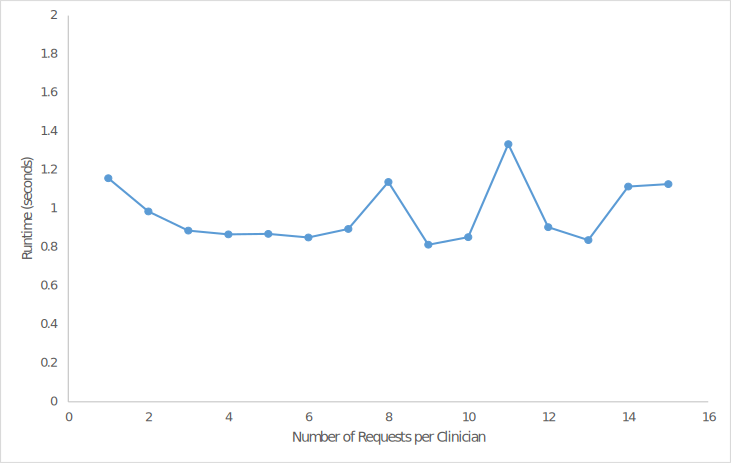
\includegraphics[scale=.5]{fig/runtime_requests} % JK: can you export this to PDF or SVG to avoid pixelation?
	\caption{Runtime of ILP solver with an increasing number of requests per clinician}
  \label{fig:runtime-requests}
  % JK: The trend here is a bit confusing, since I think you're trying to say
  %     that the runtime is not affected by the number of constraints,
  %     but there is noise in these results.
  %     I would re-run this 10-100 times and average the results so that (I expect)
  %     the mean trend is actually flat. You could (should) then also present the runtimes
  %     as box-plots to show that the trend is less than the variability.
\end{figure}

% JK: Introduce what you did first and then the figure showing results (see above)
% JK: Try to introduce these results in the same order as they appear in the
%     first paragraph of this section.
Figure~\ref{fig:runtime-blocks} presents the change in runtime when increasing
the number of 2-week blocks $B = \{26, 52, 78, 104\}$ in a department with 10
clinicians offering two services. There does not seem to be a strong effect on
runtime when we lengthen the time-horizon of the schedule, and in fact the
solver was able to find an optimal schedule for all time horizons within 3
seconds. % 'very reasonable amount of time" is vague. what is reasonable?
%better to give a range in value.
% JK: same comment as above re. trends

\begin{figure}[h]
	\centering
	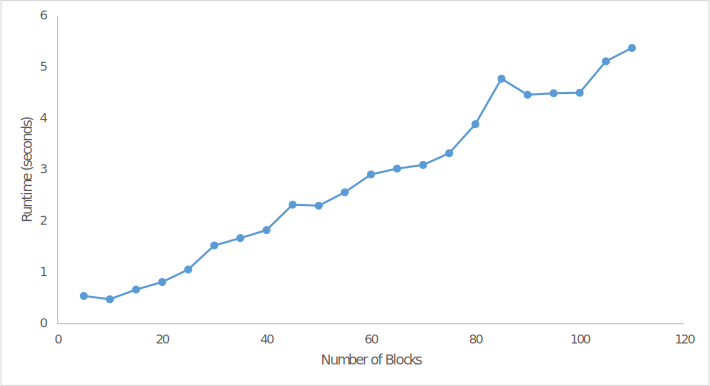
\includegraphics[scale=.5]{fig/runtime_blocks}
	\caption{Runtime of ILP solver with an increasing number of 2-week blocks}%
  \label{fig:runtime-blocks}
  % JK: same comment as above re. trends
  % JK: Thess figures could also possible be Figure 1. a) and b) 
\end{figure}
	\section{Discussion}\label{sec:discussion}
	In this paper, we present a simple, yet flexible, integer linear programming
formulation to generate schedules for clinical departments at hospitals.
The challenge in applying ILP to the task of scheduling clinicians lies in the
computational complexity of finding an optimal solution. As the size of the
scheduling problem grows, due to a larger roster of clinicians or more
complicated constraints, the time it takes to generate an optimal schedule may
grow exponentially.
%The challenge in applying such an approach to this task lies in the fact that
%ILP is an NP-hard problem. %specify what 'such an approach' and 'this task'
%are... the first part of the sentence was a bit hard to follow. Define what you
%mean by NP-hard problem and cite --> i.e. NP-hard = the following sentence
%about how time to optimal solution grows exponentially? if yes, then instead of
%'As such' - say 'That is,...or "An NP-hard problem means that..."
As a result, the majority of approaches taken to create schedules for similar
scenarios tend to use heuristics in order to find an approximately optimal
solution in a shorter time~\cite{burke_state_2004}. %cite/reference
%statement (i.e. the 'vast majority'...) I can't remember if the introduction
%details the heuristics --> but if yes, then great. if no, then include that
%review of the prior literature here in discussion. I think as you said - the
%journals we are submitting to seem to have more of those details in the
%introduction.

%double-check all abbreviations have been defined. I would prefer limiting
%abbreviations to no more than 3 at most if possible. We are ok for word count
%in this paper :). 

We presented a formulation that includes both hard constraints to ensure the
schedule satisfies hospital and logistics requirements, and a multi-goal
objective function to satisfy the work preferences of clinicians.
%Our formulation includes hard constraints to ensure the schedule satisfies
%hospital and logistics requirements. It also aims to satisfy the work
%preferences of clinicians in a clinical department by optimizing a multi-goal
%objective function. 
Although we restricted our use of the formulation to a minimal set of
constraints for the particular needs of the case study (St.\ Michael's Hospital
Division of Infectious Diseases) - our formulation can be adapted to various
clinical departments at different hospitals. The flexibility of our ILP allows
changing the number of services provided in a division, the length of a work
block, clinicians' preference for block to weekend adjacency as well as
clinicians' requests for time off.

When comparing the optimal schedule generated by our tool to the
manually-created schedules at St.\ Michael's Hospital, we found that the ILP
formulation was always able to find an optimal schedule satisfying all required
hard constraints, unlike the manual schedule, which often did not take all
constraints into account. Moreover, due to the multi-goal objective function in
the ILP, the tool was able to maximize and fulfill the majority of clinician
preferences and requests, more so than the manually-created schedule. These
observations reinforce the benefits of automated tools when generating schedules
in hospital departments to balance the work-load of clinicians and improve the
service provided to patients. The use of automated tools alleviates the time
spent on designing the schedule by hand, and provides clinical departments with
a more fair distribution of work that helps improve the overall satisfaction of
both employees and patients~\cite{silvestro_evaluation_2000}.  % how the
%finding compares to the wider literature when automated compared to manual?
%What does it mean re: "so what" - human error in generating tools, etc. or
%challenges in heuristics used manually by people? include citations this last
%sentence in particular - what dos it reinforce exactly - what are the benefits?

In our simulations, we also found that increasing the number of requests per
clinician does not affect the runtime of the algorithm, highlighting the
flexibility of the tool in incorporating clinician preferences. Further, we saw
that the algorithm can accommodate an increase in time-horizon up to four years
with little impact on runtime, which can be applied to departments that generate
schedules far in advance. One key limitation we identified was the sensitivity
of the runtime to larger numbers of services offered in a single department.
Such cases are unlikely to be encountered in the real-world because most
clinical departments tend to provide a single service or at most two services by
the same roster of clinicians [{\color{red}SM/Kevin, could you help with
	reference here?}]. One solution to mitigate the runtime issues created by a
larger number of services would be relaxing the constraints that prevent
assignment of consecutive blocks, followed by manual readjustment from the
generated schedule. %what do we mean by certain constraints? specify the other
%constraints?
Overall, our sensitivity analyses using simulated data provide reassurance that
the ILP formulation can be applied to schedule clinicians across real-world
variability between clinical departments. %SM - will look for reference and we
%can ask Kevin Gough too.
Next steps include expanding the generalizability of the tool beyond smaller
clinical departments to larger departments within and outside of health-care -
especially those that provide multiple services in parallel for patients and
other clients. 

	\section{Acknowledgements}\label{sec:acknowledgements}
	The authors are grateful to Julie Veitch (St.\ Michael's Hospital) for her contributions to testing and
designing the scheduling software. SM is supported by a Canadian Institutes of
Health Research New Investigator Award. JK is supported by a Natural Sciences and 
Engineering Research Council doctoral award. DL conducted part of this project as a
Keenan Research Summer Student, Li Ka Shing Knowledge Institute, St.\ Michael's
Hospital, University of Toronto.

	\section{Funding}\label{sec:funding}
	The work was jointly funded by the Ontario Ministry of Science and Innovation Early Researcher Award Number ER17-13-043; the Division of Infectious Diseases, St. Michael’s Hospital, University of Toronto; and the University of Toronto Work Study Program.
	
	\bibliographystyle{unsrt}
	\bibliography{references}
\end{document}
